%# -*- coding: utf-8-unix -*-
%%==================================================
%% chapter02.tex for SJTU Master Thesis
%% based on CASthesis
%% modified by wei.jianwen@gmail.com
%% Encoding: UTF-8
%%==================================================

\chapter{建模与分析}
\label{chap:example}
我们首先定义锁K的吞吐率为单位时间内K在竞争K的线程间的的平均传递次数,定义单个线程T的吞吐率为单位时间内K在T上的平均传递次数。此外,本文中锁K的长期公平性指的是长远来看,各个线程的拿锁次数之间的差异程度,可以用变异系数来衡量,变异系数越小,长期公平性越好。线程放置策略决定了线程在NUMA节点之间的分布,进而影响锁在NUMA架构机器上的吞吐率。而对于层级锁来说,由于其本地偏好的锁传递规则的影响,线程放置策略还会影响其长期公平性。本章以两层的MCS锁即C-MCS锁为例,首先通过实验验证紧凑策略和平均策略在基于队列的层级锁的吞吐率和长期公平性方面的表现,然后建模分析线程放置策略影响吞吐率和长期公平性的根本因素,进而得出线程放置策略优化应遵循的原则和面临的挑战。

\section{实验验证}
我们的实验跑在Intel Xeon E5上,该机器由四个NUMA节点组成,每个节点上包含八个计算核心。实验的benchmark取自libslock中的stress\_one,实验中用到的锁是C-MCS锁,该锁是一个两层的MCS锁,包括一个全局MCS锁和每个节点上的本地MCS锁。实验中stress\_one被配置为使用12个线程,每个线程重复以下操作:拿锁,写一定大小的缓存,放锁,暂停一段时间。该实验中我们用暂停时间的长短来控制锁的竞争强度的大小,暂停时间越短,锁的竞争越激烈,实验中用到了两个暂停
时\begin{table}[!hpb]
  \centering
  \bicaption[吞吐率对照]
    {吞吐率(acquisitions/s)}
    {Aggregate Throughput}
  \label{tab:aggregate}
  \begin{tabular}{@{}llr@{}} \toprule
    暂停时长 & 紧凑放置 & 平均放置\\ \midrule
    5000 cycles & 4574093 & 3101512 \\
    500  cycles & 4401877 & 4273903\\
  \end{tabular}
\end{table}
间:500时钟周期和5000时钟周期。图\ref{Fig:compact}和图\ref{Fig:even}分别展示了该实验在紧凑和平均(AHMCS中将平均放置到所有节点上,而本实验中也是平均放置,但为了获得更高吞吐率,我们是只使用了两个节点)两种放置策略下单个线程的吞吐率,其中在平均放置策略中我们只是用了4个NUMA节点中的两个节点。上述两张实验图中每个长条代表单个线程的吞吐率,而不同颜色表示不同的竞争强度。表\ref{tab:aggregate}和表\ref{tab:CV}分别显示了不同配置下的吞吐率及变异系数。

\begin{table}[!hpb]
  \centering
  \bicaption[变异系数对照]
    {变异系数}
    {Coefficient of Variance}
  \label{tab:CV}
  \begin{tabular}{@{}llr@{}} \toprule
    暂停时长 & 紧凑放置 & 平均放置\\ \midrule
    5000 cycles & 64.174778\% & 1.939154\%\\
    500  cycles & 35.315475\% & 0.036318\%\\
  \end{tabular}
\end{table}

从表\ref{tab:aggregate}中可以看出,两种竞争强度下的最高吞吐率比较接近,即增加单个线程的锁请求频率并未增加吞吐率,所以上述两种竞争强度下C-MCS锁都已经达到了饱和。在锁达到饱和并且关键区域执行时间不变的情况下,影响吞吐率的最主要的因素将是锁传递的平均时延大小,而在NUMA架构下影响锁传递平均时延大小的主要是锁在NUMA节点之间传递的频率。

结合图\ref{Fig:compact}、表\ref{tab:aggregate}和表\ref{tab:CV}可以看出紧凑放置能够尽可能地保证层级锁的高吞吐率,但是吞吐率在线程之间地分布是严重不均衡的,同一个NUMA节点上的线程吞吐率基本相同,不同NUMA节点上地线程之间吞吐率差别可以达到十几倍,而且实验中的两种竞争强度下受益的线程集合正好相反。结合图\ref{Fig:even}、表\ref{tab:aggregate}和表\ref{tab:CV}可以看出平均放置能够保证层级锁的长期公平性,单个线程的吞吐率之间没有明显的差异,但是即使在总的竞争已经饱和而且在平均放置的基础上使线程放置地尽可能地紧凑的情况下,如果竞争并不是很高其总的吞吐率相比紧凑放置还是有明显地损失,实验中其总吞吐率损失多大32.2\%。

\begin{figure}[t]
	\centering
	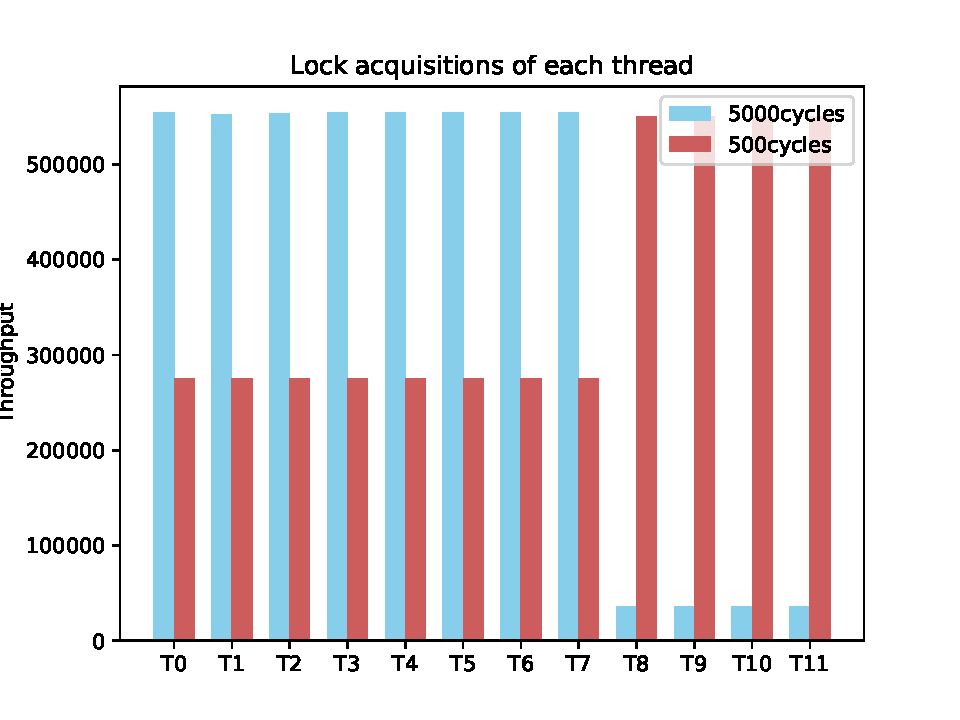
\includegraphics[width=5.6in]{compact.pdf}
	\caption{紧凑放置:单个线程的吞吐率}
	\label{Fig:compact}
\end{figure}

\begin{figure}[t]
	\centering
	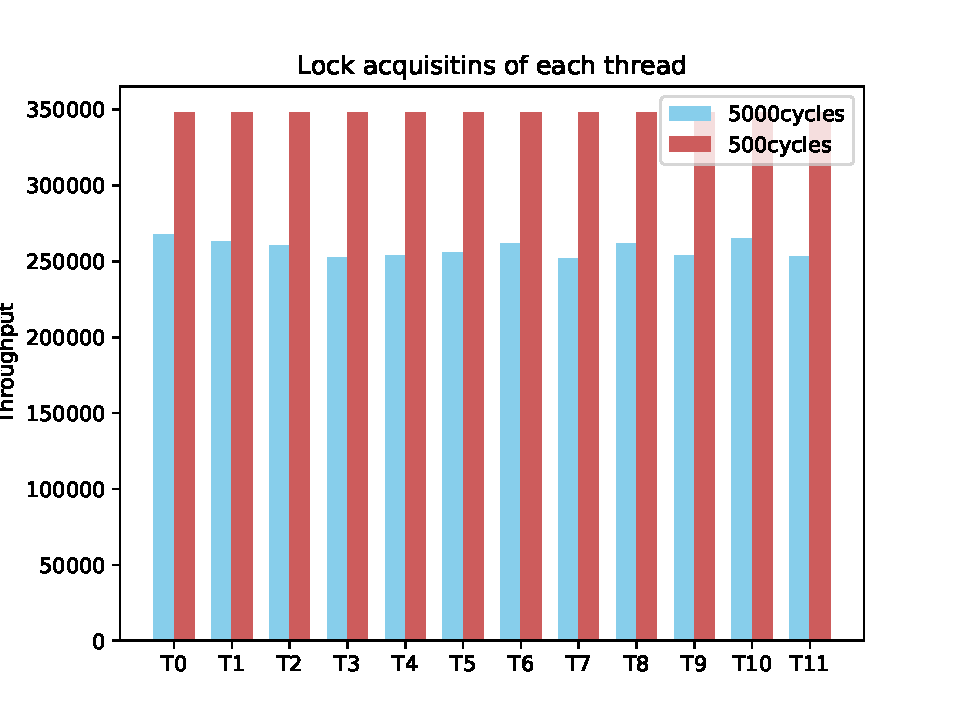
\includegraphics[width=5.6in]{even.pdf}
	\caption{平均放置:单个线程的吞吐率}
	\label{Fig:even}
\end{figure}

\section{建模}
本小节中我们以C-MCS锁为例,通过建模从微观角度分析线程放置策略中影响基于队列的层级锁的总吞吐率和长期公平性的关键因素。

\begin{figure}[t]
	\centering
	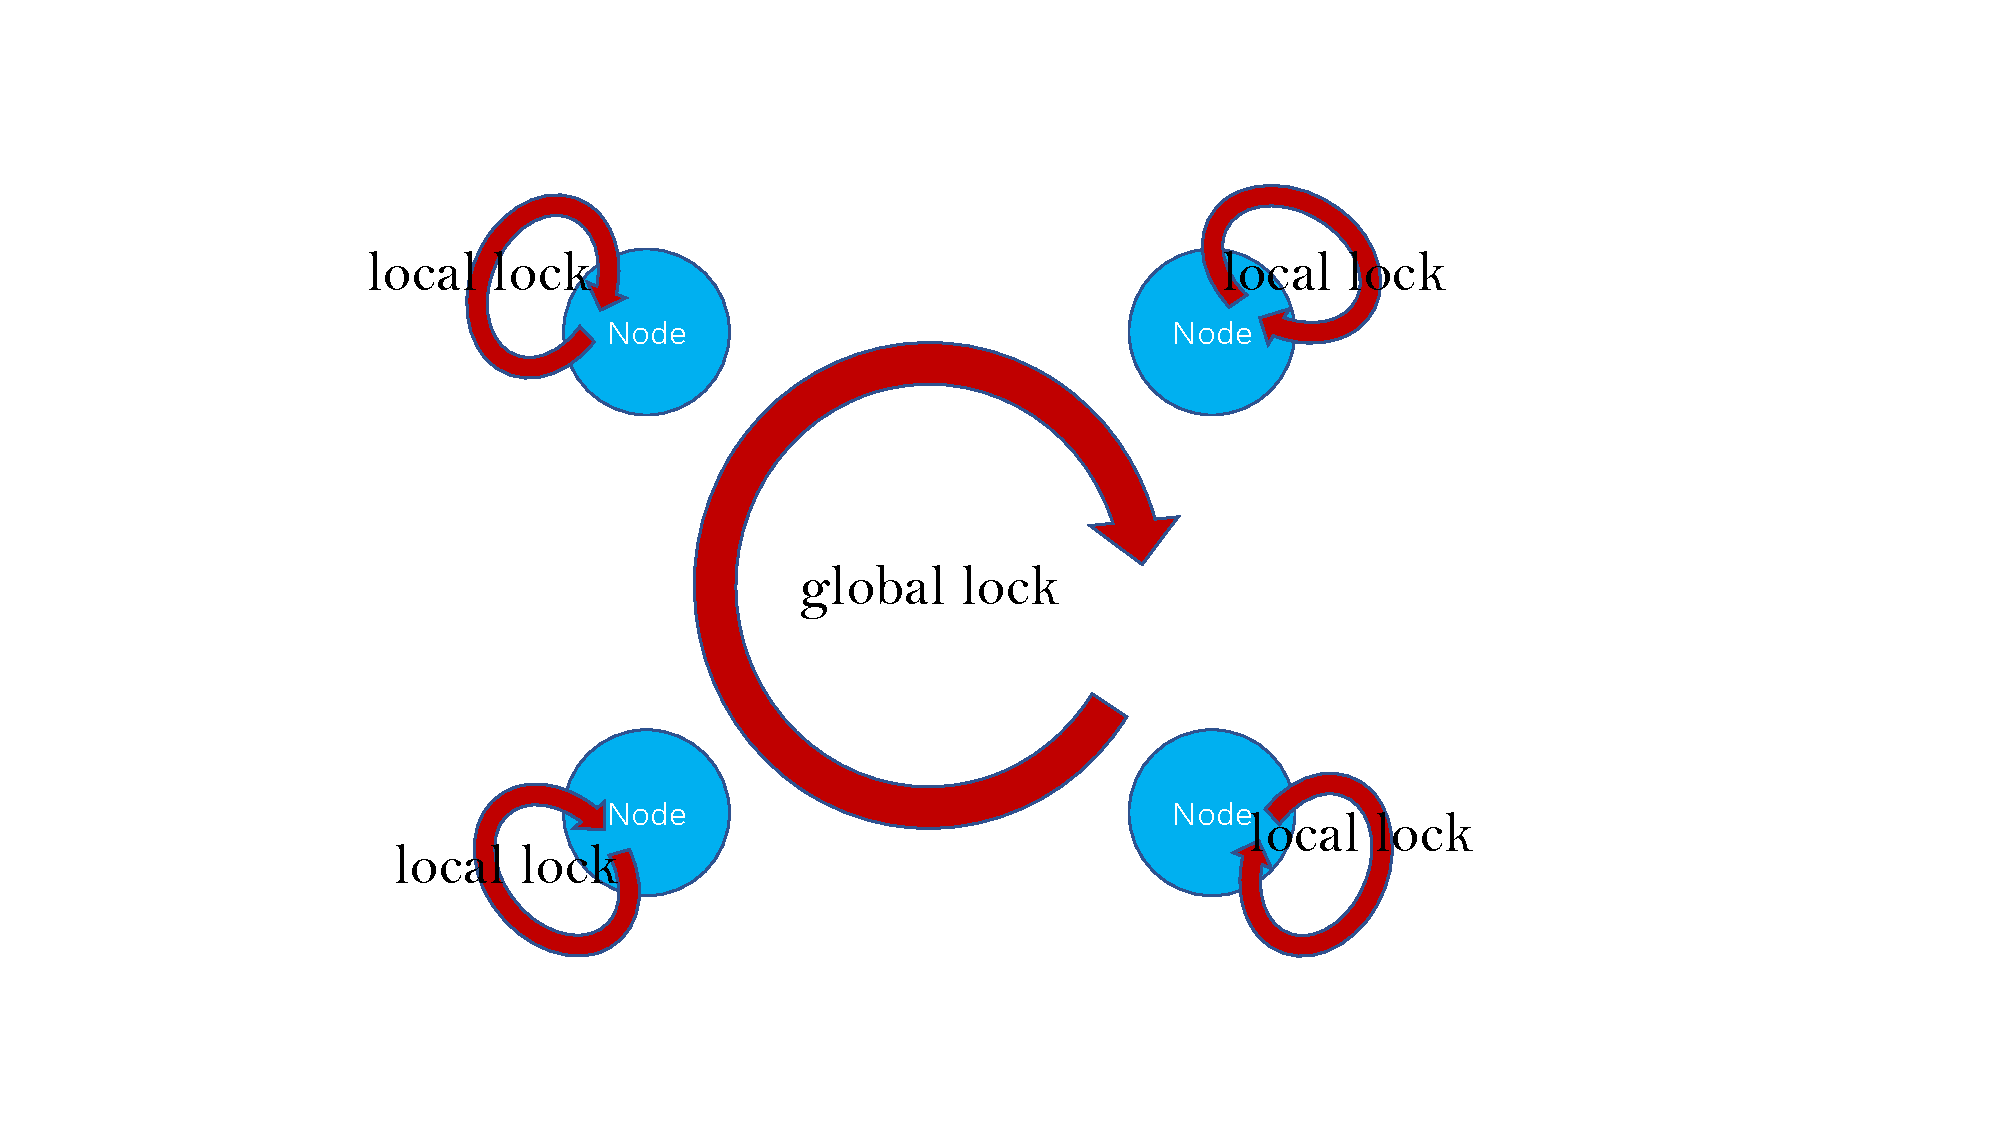
\includegraphics[width=5.6in]{circulation.pdf}
	\caption{C-MCS锁中的一个循环}
	\label{Fig:circulation}
\end{figure}

因为层级锁主要用于竞争线程较多竞争较激烈的场景,所以以下建模分析基于层级锁的竞争较为激烈至少已经饱和的假设。C-MCS锁中用到的全局锁和本地锁都是MCS锁,而MCS锁按照先进先出(FIFO,first in first out)的顺序在线程之间传递,所以我们可以认为全局MCS锁在相关NUMA节点之间按照round-robin的方式传递;对于某个特定节点上的线程来说,当第一个请求者代表该节点拿到全局锁时,对应的本地MCS锁在该节点上运行的所有相关节点之间也按round-Robin的方式传递,直到最后一个请求者释放全局锁(当前节点没有后续请求者)或者某个请求者被强制释放全局锁(当前节点上的传递次数达到threshold),如图\ref{Fig:circulation}所示。为了说明的方便,我们将全局MCS锁在所有相关节点之间传递一次的时间间隔定义为一个循环(circulation),并且以一个循环为单位来评估吞吐率和长期公平性。


我们用N表示竞争锁的线程数,这些线程分布在S个节点上,大小为S数组Count中每个元素Count[i]表示节点i上放置的线程数,则有约束:
\begin{equation}\label{Eq:threads}
  \sum_{i=1}^{S} Count[i] = N
\end{equation}
\begin{equation}\label{Eq:non-zero}
  Count[i] > 0 \quad for\;each\;  i\; in\; 1\;to\;S
\end{equation}
其中S及Count数组中每个元素的大小都是由线程放置策略决定的,只要满足上述约束即可。我们用大小为N的数组Acquisitions中每个元素Acquisitions[i]表示线程i在一个循环内的拿锁次数,用interl表示跨节点的锁传递时延,用intral表示同一节点内的锁传递时延,则一个循环的总时间可以表示为
\begin{equation}\label{Eq:duration}
 Duration=\sum_{i=1}^{N} Acquisitions[i] * intral + S * (interl - intral)
\end{equation}
一个循环内总的锁传递次数可以表示为
\begin{equation}\label{Eq:totalacqui}
  TotalAcquisitions=\sum_{i=1}^{N} Acquisitions[i]
\end{equation}
进而吞吐率可以表示为
\begin{equation}\label{Eq:total-thrpt}
 Throughput=\frac{TotalAcquisitions}{Duration}
\end{equation}
一个循环内每个线程的平均拿锁次数为
\begin{equation}\label{Eq:AVG}
  \mu = \frac{TotalAcquisitions}{N}
\end{equation}
标准差为
\begin{equation}\label{Eq:SD}
  \sigma=\sqrt{\frac{\sum_{i=1}^N(Acquisitions[i]-\mu)^2}{N}}
\end{equation}
而变异系数可以表示为
\begin{equation}\label{Eq:CV}
 c_v=\frac{\sigma}{\mu}
\end{equation}

由式\ref{Eq:duration}到式\ref{Eq:total-thrpt}可知$\sum_{i=1}^{N} Acquisitions[i]$越大,即一个循环内总的锁传递次数越多,吞吐率越高;而由式\ref{Eq:totalacqui}、式\ref{Eq:AVG}和式\ref{Eq:CV}可知,Acquisitions中N个元素越接近,即N个线程的拿锁次数之间的差异越小,变异系数越小,长期公平性越好。故吞吐率和变异系数都与一个循环内每个线程的拿锁次数有关,所以以下我们按照C-MCS锁的传递规则对一个循环内每个元素的拿锁次数Acquisitions[i]进行建模。

对于只有一个线程的应用来说,其任何时刻在执行关键区域的概率可以表述为:
\begin{equation}\label{Eq:pro}
     P_{cs} = CS / (NCS + CS)
\end{equation}
其中CS和NCS分别代表关键区域和非关键区域的长度。那么对一个包含T个请求同一个锁的线程的应用来说,其任何时刻在执行或者等待执行关键区域的线程数的期望值为:
\begin{equation}\label{Eq:expectation}
     E_{cs} = T * P_{cs}
\end{equation}
\emph{Ecs}由应用中锁的竞争者的数量和单个竞争者请求锁的频率计算而来,可以用来表示和评估应用中的锁的总体竞争强度,Ecs越大意味着锁被请求的越频繁,即锁的竞争越激烈。当\emph{Ecs}的值为1时,锁被持续持有并且所有线程无需等待就能在请求锁的时候就拿到锁,如图\ref{Fig:saturation}所示,此时的线程数即为该锁当前的饱和点\cite{dice2017malthusian}。由式\ref{Eq:expectation}可得饱和点的值可以表示如下
\begin{equation}\label{Eq:sat}
     Sat = (NCS + CS) / CS
\end{equation}

\begin{figure}[t]
	\centering
	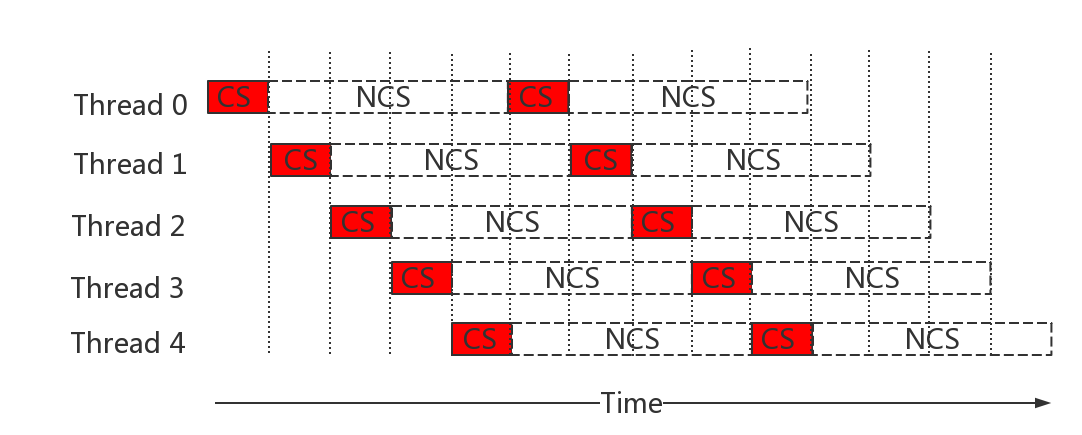
\includegraphics[width=5.6in]{saturation.png}
	\caption{饱和点,该图示中饱和点为5}
	\label{Fig:saturation}
\end{figure}

现在考虑C-MCS锁的传递规则,在每一个循环中,如果NUMA节点k上的线程数Count[k]大于等于饱和点Sat,则节点k上的任何一个线程在放锁时总是至少有一个线程在等待锁,所以锁会在该节点上一直传递直到节点k上总的传递次数达到预先设定的上限threshold;否则节点k上的最后一个线程放锁后其他线程还在执行非关键区域,故一个循环内锁在该节点上的传递次数为Count[k]。即
\begin{equation}\label{Eq:localtrans}
node\_acquisitions =
\begin{cases}
Count[k] &\text{Count[k] < Sat}\\
threshold &\text{otherwise}
\end{cases}
\end{equation}
因为每个节点上的本地MCS锁是完全公平的,所以我们可以认为同一个节点上的每个线程的在一个循环内的拿锁次数相等,即节点k上每个线程i在一个循环里边的拿锁次数为
\begin{equation}\label{Eq:per}
Acquisitions[i] =
\begin{cases}
1 &\text{Count[k] < Sat}\\
\frac{threshold}{Count[k]} &\text{otherwise}
\end{cases}
\end{equation}
一般情况下为了获取更高的吞吐率,threshold通常被设为Count[k]的若干倍,所以每个节点上放置的线程能否使该节点上的本地锁饱和对于该节点上的每个线程在一个循环内的拿锁次数影响很大。

\section{模型分析}
基于上述建模,我们可以得出下述结论:
\begin{itemize}
    \item 吞吐率由一个循环内总的锁传递次数决定,一个循环内总的所传递次数越多,吞吐率越高;
    \item 长期公平性由一个循环内各个线程拿锁次数之间的离散程度决定,各个线程拿锁次数越接近,长期公平性越好;
    \item 一个循环内同一个节点内的线程的拿锁次数相等;
    \item 一个循环内两个不同节点l和m上的线程的拿锁次数是否相等由Count[l]和Count[m]是否相等决定的;
    \item 节点k上放置的线程数Count[k]与饱和点Sat的关系决定了一个循环内节点k上每个线程的拿锁次数是1还是$\frac{threshold}{Count[k]}$,并且一般情况下threshold被设置为Count[k]的若干倍。
\end{itemize}
所以在基于队列的层级锁中获取尽可能高吞吐率的一个充分条件是保证尽可能多的节点上放置的线程数大于等于饱和点Sat;而保证长期公平性的一个充分条件是使所有节点上放置的线程数相等。本章开头的实验中紧凑放置在竞争较小时(此时Sat较大)相比平均放置能够获得更高吞吐率的原因就在于,此时紧凑放置至少保证了一个节点上放置的线程数大于等于饱和点,而平均放置中两个节点上放置的线程数都小于饱和点;紧凑放置在两种竞争强度下都不能保证长期公平性的原因则在于两个节点上放置的线程数不相等。

\begin{figure}[t]
	\centering
	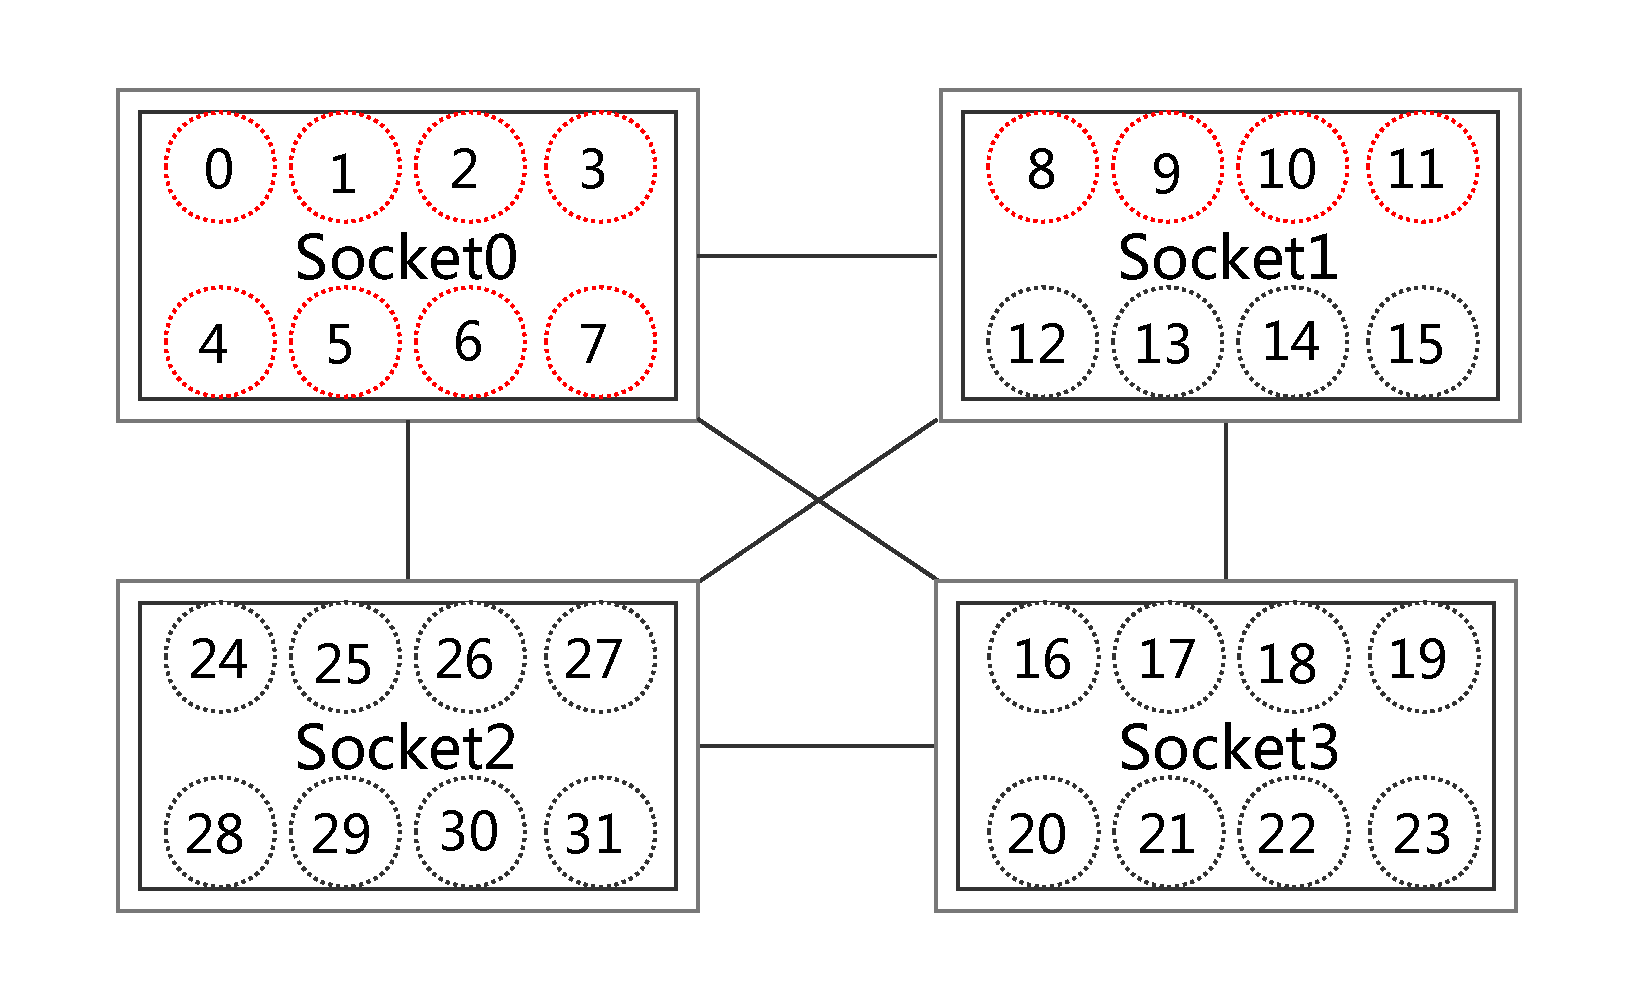
\includegraphics[width=5.6in]{symmetric.pdf}
	\caption{线程等价类}
	\label{Fig:symmetric}
\end{figure}

为了进一步说明线程放置对基于队列的锁的长期公平性的影响,我们定义两个线程之间的关系为对称(symmetric)如果不管锁的竞争强度如何变化,这两个线程理论上长期的拿锁次数差距为0。由上述建模及分析可知,运行在同一个NUMA节点上的任何两个线程之间是对称的;而对于运行在两个不同节点上的线程来说,当这两个节点上运行的线程数量相等时,这两个线程是对称的。显然,对称关系是一种等价关系,因此所有竞争同一个层级锁的线程可以按照其在NUMA节点上的分布来被分为若干等价类。例如,图\ref{Fig:symmetric}中的20个线程可以分为两个等价类,其中节点0上的8个线程和节点3上的8个线程属于同一个等价类,剩下的4个线程属于另一个等价类。所以我们也可以说保证基于队列的层级锁的长期公平性的一个充分条件是使所有线程按照对称关系属于同一个等价类。

\section{挑战分析}
从上述建模和分析可以看出从线程放置的角度保证基于队列的层级锁的吞吐率和长期公平性两者之一是非常简单直接的,但是同时保证两者则要面临以下限制挑战:
\begin{enumerate}
  \item 节点k上可以放置的线程数Count[k]应该小于等于节点k上的计算核心数,否则可能会产生锁的持有者或等待着被抢占的问题;
  \item 应用中的线程数和饱和点都可能随着上层的业务需求和下层的硬件资源状况变化,简单单一的线程放置策略只能在某些情况下同时保证高吞吐量和长期公平性;
  \item 受制于单个节点上所能放置的线程数,保证每个节点上的放置的线程数相等和保证尽可能多的节点上放置的线程数大于等于饱和点这两个目标有时候很难同时达到。
\end{enumerate}

在公有云等很多共享资源的场景下,资源的高效利用和资源在用户间的公平分配对于其的成功同等重要;这些应用场景同时也因为价格、时段等因素的影响,资源的需求变化很大,再加上多种应用共享底层硬件资源带来的影响,使得共享资源的竞争很难预测和控制。这些都对共享资源的分配和利用提出了新的挑战,从本章的分析可以看出线程放置对于使用层级锁的应用中的共享资源的利用和其在线程间的分配有很大影响。而现有的简单单一的线程放置策略不能满足应用在各种复杂多变的需求下对层级锁吞吐率和长期公平性的需求,我们需要额外的技术和更复杂更合理更细力度的线程放置策略来应对这些挑战。

\section{本章小结}
在这一章中,我们首先通过实验展示了现有基于队列的层级锁中线程放置策略在吞吐率和长期公平性方面的存在的缺陷,然后通过对吞吐率和长期公平性建模分析出了决定基于队列的层级锁的吞吐率和长期公平性的关键因素,最后在此基础山得出了基于队列的层级锁中线程放置策略所面临的挑战,从而为后续说明竞争感知的混合线程放置策略做好了理论基础。